\documentclass[1p]{elsarticle_modified}
%\bibliographystyle{elsarticle-num}

%\usepackage[colorlinks]{hyperref}
%\usepackage{abbrmath_seonhwa} %\Abb, \Ascr, \Acal ,\Abf, \Afrak
\usepackage{amsfonts}
\usepackage{amssymb}
\usepackage{amsmath}
\usepackage{amsthm}
\usepackage{scalefnt}
\usepackage{amsbsy}
\usepackage{kotex}
\usepackage{caption}
\usepackage{subfig}
\usepackage{color}
\usepackage{graphicx}
\usepackage{xcolor} %% white, black, red, green, blue, cyan, magenta, yellow
\usepackage{float}
\usepackage{setspace}
\usepackage{hyperref}

\usepackage{tikz}
\usetikzlibrary{arrows}

\usepackage{multirow}
\usepackage{array} % fixed length table
\usepackage{hhline}

%%%%%%%%%%%%%%%%%%%%%
\makeatletter
\renewcommand*\env@matrix[1][\arraystretch]{%
	\edef\arraystretch{#1}%
	\hskip -\arraycolsep
	\let\@ifnextchar\new@ifnextchar
	\array{*\c@MaxMatrixCols c}}
\makeatother %https://tex.stackexchange.com/questions/14071/how-can-i-increase-the-line-spacing-in-a-matrix
%%%%%%%%%%%%%%%

\usepackage[normalem]{ulem}

\newcommand{\msout}[1]{\ifmmode\text{\sout{\ensuremath{#1}}}\else\sout{#1}\fi}
%SOURCE: \msout is \stkout macro in https://tex.stackexchange.com/questions/20609/strikeout-in-math-mode

\newcommand{\cancel}[1]{
	\ifmmode
	{\color{red}\msout{#1}}
	\else
	{\color{red}\sout{#1}}
	\fi
}

\newcommand{\add}[1]{
	{\color{blue}\uwave{#1}}
}

\newcommand{\replace}[2]{
	\ifmmode
	{\color{red}\msout{#1}}{\color{blue}\uwave{#2}}
	\else
	{\color{red}\sout{#1}}{\color{blue}\uwave{#2}}
	\fi
}

\newcommand{\Sol}{\mathcal{S}} %segment
\newcommand{\D}{D} %diagram
\newcommand{\A}{\mathcal{A}} %arc


%%%%%%%%%%%%%%%%%%%%%%%%%%%%%5 test

\def\sl{\operatorname{\textup{SL}}(2,\Cbb)}
\def\psl{\operatorname{\textup{PSL}}(2,\Cbb)}
\def\quan{\mkern 1mu \triangleright \mkern 1mu}

\theoremstyle{definition}
\newtheorem{thm}{Theorem}[section]
\newtheorem{prop}[thm]{Proposition}
\newtheorem{lem}[thm]{Lemma}
\newtheorem{ques}[thm]{Question}
\newtheorem{cor}[thm]{Corollary}
\newtheorem{defn}[thm]{Definition}
\newtheorem{exam}[thm]{Example}
\newtheorem{rmk}[thm]{Remark}
\newtheorem{alg}[thm]{Algorithm}

\newcommand{\I}{\sqrt{-1}}
\begin{document}

%\begin{frontmatter}
%
%\title{Boundary parabolic representations of knots up to 8 crossings}
%
%%% Group authors per affiliation:
%\author{Yunhi Cho} 
%\address{Department of Mathematics, University of Seoul, Seoul, Korea}
%\ead{yhcho@uos.ac.kr}
%
%
%\author{Seonhwa Kim} %\fnref{s_kim}}
%\address{Center for Geometry and Physics, Institute for Basic Science, Pohang, 37673, Korea}
%\ead{ryeona17@ibs.re.kr}
%
%\author{Hyuk Kim}
%\address{Department of Mathematical Sciences, Seoul National University, Seoul 08826, Korea}
%\ead{hyukkim@snu.ac.kr}
%
%\author{Seokbeom Yoon}
%\address{Department of Mathematical Sciences, Seoul National University, Seoul, 08826,  Korea}
%\ead{sbyoon15@snu.ac.kr}
%
%\begin{abstract}
%We find all boundary parabolic representation of knots up to 8 crossings.
%
%\end{abstract}
%\begin{keyword}
%    \MSC[2010] 57M25 
%\end{keyword}
%
%\end{frontmatter}

%\linenumbers
%\tableofcontents
%
\newcommand\colored[1]{\textcolor{white}{\rule[-0.35ex]{0.8em}{1.4ex}}\kern-0.8em\color{red} #1}%
%\newcommand\colored[1]{\textcolor{white}{ #1}\kern-2.17ex	\textcolor{white}{ #1}\kern-1.81ex	\textcolor{white}{ #1}\kern-2.15ex\color{red}#1	}

{\Large $\underline{12a_{1147}~(K12a_{1147})}$}

\setlength{\tabcolsep}{10pt}
\renewcommand{\arraystretch}{1.6}
\vspace{1cm}\begin{tabular}{m{100pt}>{\centering\arraybackslash}m{274pt}}
\multirow{5}{120pt}{
	\centering
	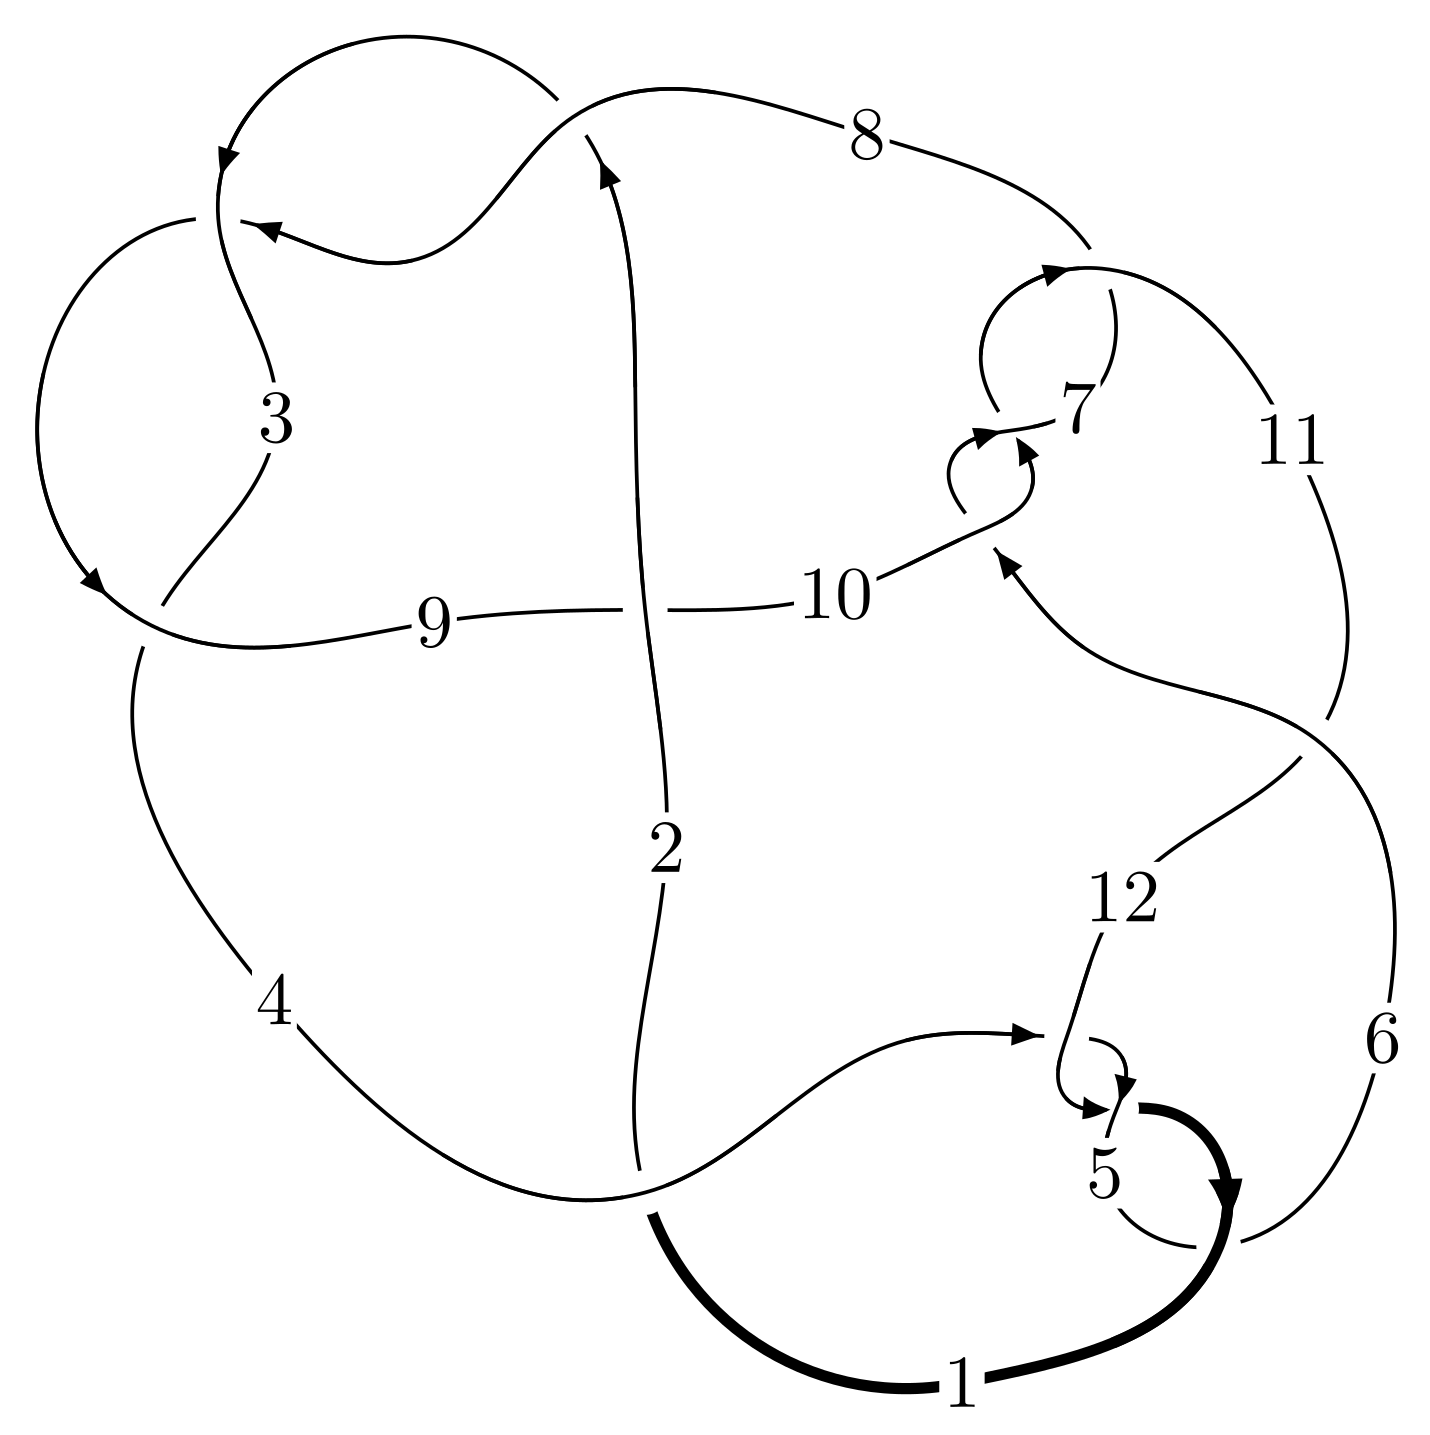
\includegraphics[width=112pt]{../../../GIT/diagram.site/Diagrams/png/1948_12a_1147.png}\\
\ \ \ A knot diagram\footnotemark}&
\allowdisplaybreaks
\textbf{Linearized knot diagam} \\
\cline{2-2}
 &
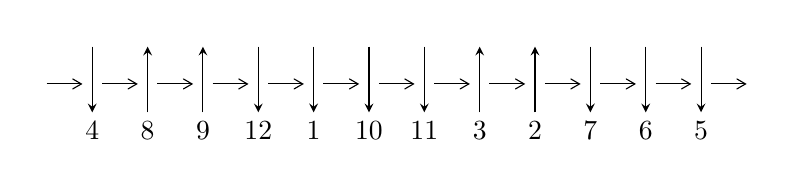
\begin{tikzpicture}[x=20pt, y=17pt]
	% nodes
	\node (C0) at (0, 0) {};
	\node (C1) at (1, 0) {};
	\node (C1U) at (1, +1) {};
	\node (C1D) at (1, -1) {4};

	\node (C2) at (2, 0) {};
	\node (C2U) at (2, +1) {};
	\node (C2D) at (2, -1) {8};

	\node (C3) at (3, 0) {};
	\node (C3U) at (3, +1) {};
	\node (C3D) at (3, -1) {9};

	\node (C4) at (4, 0) {};
	\node (C4U) at (4, +1) {};
	\node (C4D) at (4, -1) {12};

	\node (C5) at (5, 0) {};
	\node (C5U) at (5, +1) {};
	\node (C5D) at (5, -1) {1};

	\node (C6) at (6, 0) {};
	\node (C6U) at (6, +1) {};
	\node (C6D) at (6, -1) {10};

	\node (C7) at (7, 0) {};
	\node (C7U) at (7, +1) {};
	\node (C7D) at (7, -1) {11};

	\node (C8) at (8, 0) {};
	\node (C8U) at (8, +1) {};
	\node (C8D) at (8, -1) {3};

	\node (C9) at (9, 0) {};
	\node (C9U) at (9, +1) {};
	\node (C9D) at (9, -1) {2};

	\node (C10) at (10, 0) {};
	\node (C10U) at (10, +1) {};
	\node (C10D) at (10, -1) {7};

	\node (C11) at (11, 0) {};
	\node (C11U) at (11, +1) {};
	\node (C11D) at (11, -1) {6};

	\node (C12) at (12, 0) {};
	\node (C12U) at (12, +1) {};
	\node (C12D) at (12, -1) {5};
	\node (C13) at (13, 0) {};

	% arrows
	\draw[->,>={angle 60}]
	(C0) edge (C1) (C1) edge (C2) (C2) edge (C3) (C3) edge (C4) (C4) edge (C5) (C5) edge (C6) (C6) edge (C7) (C7) edge (C8) (C8) edge (C9) (C9) edge (C10) (C10) edge (C11) (C11) edge (C12) (C12) edge (C13) ;	\draw[->,>=stealth]
	(C1U) edge (C1D) (C2D) edge (C2U) (C3D) edge (C3U) (C4U) edge (C4D) (C5U) edge (C5D) (C6U) edge (C6D) (C7U) edge (C7D) (C8D) edge (C8U) (C9D) edge (C9U) (C10U) edge (C10D) (C11U) edge (C11D) (C12U) edge (C12D) ;
	\end{tikzpicture} \\
\hhline{~~} \\& 
\textbf{Solving Sequence} \\ \cline{2-2} 
 &
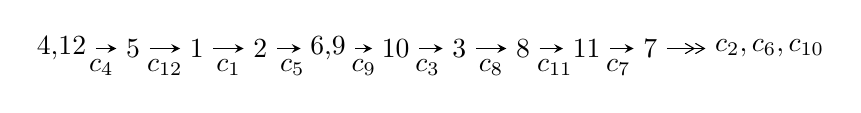
\begin{tikzpicture}[x=23pt, y=7pt]
	% node
	\node (A0) at (-1/8, 0) {4,12};
	\node (A1) at (1, 0) {5};
	\node (A2) at (2, 0) {1};
	\node (A3) at (3, 0) {2};
	\node (A4) at (65/16, 0) {6,9};
	\node (A5) at (41/8, 0) {10};
	\node (A6) at (49/8, 0) {3};
	\node (A7) at (57/8, 0) {8};
	\node (A8) at (65/8, 0) {11};
	\node (A9) at (73/8, 0) {7};
	\node (C1) at (1/2, -1) {$c_{4}$};
	\node (C2) at (3/2, -1) {$c_{12}$};
	\node (C3) at (5/2, -1) {$c_{1}$};
	\node (C4) at (7/2, -1) {$c_{5}$};
	\node (C5) at (37/8, -1) {$c_{9}$};
	\node (C6) at (45/8, -1) {$c_{3}$};
	\node (C7) at (53/8, -1) {$c_{8}$};
	\node (C8) at (61/8, -1) {$c_{11}$};
	\node (C9) at (69/8, -1) {$c_{7}$};
	\node (A10) at (11, 0) {$c_{2},c_{6},c_{10}$};

	% edge
	\draw[->,>=stealth]	
	(A0) edge (A1) (A1) edge (A2) (A2) edge (A3) (A3) edge (A4) (A4) edge (A5) (A5) edge (A6) (A6) edge (A7) (A7) edge (A8) (A8) edge (A9) ;
	\draw[->>,>={angle 60}]	
	(A9) edge (A10);
\end{tikzpicture} \\ 

\end{tabular} \\

\footnotetext{
The image of knot diagram is generated by the software ``\textbf{Draw programme}" developed by Andrew Bartholomew(\url{http://www.layer8.co.uk/maths/draw/index.htm\#Running-draw}), where we modified some parts for our purpose(\url{https://github.com/CATsTAILs/LinksPainter}).
}\phantom \\ \newline 
\centering \textbf{Ideals for irreducible components\footnotemark of $X_{\text{par}}$} 
 
\begin{align*}
I^u_{1}&=\langle 
- u^{22}- u^{21}+\cdots+2 b+1,\;u^{22}+u^{21}+\cdots+2 a-1,\;u^{24}+u^{23}+\cdots+u^2+1\rangle \\
I^u_{2}&=\langle 
663778 u^{39}+3468564 u^{38}+\cdots+4497023 b+12669528,\\
\phantom{I^u_{2}}&\phantom{= \langle  }1460252 u^{39}+3892416 u^{38}+\cdots+4497023 a+44643349,\;u^{40}+u^{39}+\cdots+10 u-1\rangle \\
I^u_{3}&=\langle 
b,\;a+1,\;u+1\rangle \\
I^u_{4}&=\langle 
b+a-1,\;a^2-2 a-1,\;u-1\rangle \\
\\
\end{align*}
\raggedright * 4 irreducible components of $\dim_{\mathbb{C}}=0$, with total 67 representations.\\
\footnotetext{All coefficients of polynomials are rational numbers. But the coefficients are sometimes approximated in decimal forms when there is not enough margin.}
\newpage
\renewcommand{\arraystretch}{1}
\centering \section*{I. $I^u_{1}= \langle - u^{22}- u^{21}+\cdots+2 b+1,\;u^{22}+u^{21}+\cdots+2 a-1,\;u^{24}+u^{23}+\cdots+u^2+1 \rangle$}
\flushleft \textbf{(i) Arc colorings}\\
\begin{tabular}{m{7pt} m{180pt} m{7pt} m{180pt} }
\flushright $a_{4}=$&$\begin{pmatrix}1\\0\end{pmatrix}$ \\
\flushright $a_{12}=$&$\begin{pmatrix}0\\u\end{pmatrix}$ \\
\flushright $a_{5}=$&$\begin{pmatrix}1\\u^2\end{pmatrix}$ \\
\flushright $a_{1}=$&$\begin{pmatrix}- u\\- u^3+u\end{pmatrix}$ \\
\flushright $a_{2}=$&$\begin{pmatrix}u^3-2 u\\- u^3+u\end{pmatrix}$ \\
\flushright $a_{6}=$&$\begin{pmatrix}- u^2+1\\- u^4+2 u^2\end{pmatrix}$ \\
\flushright $a_{9}=$&$\begin{pmatrix}-\frac{1}{2} u^{22}-\frac{1}{2} u^{21}+\cdots-2 u+\frac{1}{2}\\\frac{1}{2} u^{22}+\frac{1}{2} u^{21}+\cdots- u-\frac{1}{2}\end{pmatrix}$ \\
\flushright $a_{10}=$&$\begin{pmatrix}u^3-2 u\\\frac{1}{2} u^{22}+\frac{1}{2} u^{21}+\cdots- u-\frac{1}{2}\end{pmatrix}$ \\
\flushright $a_{3}=$&$\begin{pmatrix}-\frac{1}{2} u^{22}-\frac{1}{2} u^{21}+\cdots- u+\frac{1}{2}\\-\frac{1}{2} u^{23}+\frac{11}{2} u^{21}+\cdots+\frac{3}{2} u+\frac{1}{2}\end{pmatrix}$ \\
\flushright $a_{8}=$&$\begin{pmatrix}u^6-3 u^4+2 u^2+1\\-\frac{1}{2} u^{23}-\frac{1}{2} u^{22}+\cdots+4 u^2+\frac{1}{2} u\end{pmatrix}$ \\
\flushright $a_{11}=$&$\begin{pmatrix}u^5-2 u^3+u\\u^7-3 u^5+2 u^3+u\end{pmatrix}$ \\
\flushright $a_{7}=$&$\begin{pmatrix}- u^4+u^2+1\\-\frac{1}{2} u^{23}-\frac{1}{2} u^{22}+\cdots+3 u^2+\frac{1}{2} u\end{pmatrix}$\\&\end{tabular}
\flushleft \textbf{(ii) Obstruction class $= -1$}\\~\\
\flushleft \textbf{(iii) Cusp Shapes $= -2 u^{23}- u^{22}+23 u^{21}+8 u^{20}-113 u^{19}-20 u^{18}+300 u^{17}-9 u^{16}-430 u^{15}+142 u^{14}+219 u^{13}-271 u^{12}+253 u^{11}+142 u^{10}-424 u^9+149 u^8+116 u^7-175 u^6+131 u^5-14 u^4-65 u^3+44 u^2-8 u-1$}\\~\\
\newpage\renewcommand{\arraystretch}{1}
\flushleft \textbf{(iv) u-Polynomials at the component}\newline \\
\begin{tabular}{m{50pt}|m{274pt}}
Crossings & \hspace{64pt}u-Polynomials at each crossing \\
\hline $$\begin{aligned}c_{1},c_{11}\end{aligned}$$&$\begin{aligned}
&u^{24}-3 u^{23}+\cdots+16 u-16
\end{aligned}$\\
\hline $$\begin{aligned}c_{2},c_{3},c_{8}\end{aligned}$$&$\begin{aligned}
&u^{24}-3 u^{23}+\cdots+2 u-2
\end{aligned}$\\
\hline $$\begin{aligned}c_{4},c_{5},c_{6}\\c_{7},c_{10},c_{12}\end{aligned}$$&$\begin{aligned}
&u^{24}+u^{23}+\cdots+u^2+1
\end{aligned}$\\
\hline $$\begin{aligned}c_{9}\end{aligned}$$&$\begin{aligned}
&u^{24}+9 u^{23}+\cdots-38 u-46
\end{aligned}$\\
\hline
\end{tabular}\\~\\
\newpage\renewcommand{\arraystretch}{1}
\flushleft \textbf{(v) Riley Polynomials at the component}\newline \\
\begin{tabular}{m{50pt}|m{274pt}}
Crossings & \hspace{64pt}Riley Polynomials at each crossing \\
\hline $$\begin{aligned}c_{1},c_{11}\end{aligned}$$&$\begin{aligned}
&y^{24}+17 y^{23}+\cdots-1280 y+256
\end{aligned}$\\
\hline $$\begin{aligned}c_{2},c_{3},c_{8}\end{aligned}$$&$\begin{aligned}
&y^{24}-23 y^{23}+\cdots+28 y+4
\end{aligned}$\\
\hline $$\begin{aligned}c_{4},c_{5},c_{6}\\c_{7},c_{10},c_{12}\end{aligned}$$&$\begin{aligned}
&y^{24}-23 y^{23}+\cdots+2 y+1
\end{aligned}$\\
\hline $$\begin{aligned}c_{9}\end{aligned}$$&$\begin{aligned}
&y^{24}-11 y^{23}+\cdots+7020 y+2116
\end{aligned}$\\
\hline
\end{tabular}\\~\\
\newpage\flushleft \textbf{(vi) Complex Volumes and Cusp Shapes}
$$\begin{array}{c|c|c}  
\text{Solutions to }I^u_{1}& \I (\text{vol} + \sqrt{-1}CS) & \text{Cusp shape}\\
 \hline 
\begin{aligned}
u &= \phantom{-}0.064601 + 0.857743 I \\
a &= \phantom{-}3.00242 + 0.79694 I \\
b &= -1.47055 + 0.22609 I\end{aligned}
 & \phantom{-}11.05360 - 5.17653 I & \phantom{-}3.95325 + 3.49150 I \\ \hline\begin{aligned}
u &= \phantom{-}0.064601 - 0.857743 I \\
a &= \phantom{-}3.00242 - 0.79694 I \\
b &= -1.47055 - 0.22609 I\end{aligned}
 & \phantom{-}11.05360 + 5.17653 I & \phantom{-}3.95325 - 3.49150 I \\ \hline\begin{aligned}
u &= -0.034624 + 0.810902 I \\
a &= -1.048330 - 0.309670 I \\
b &= \phantom{-}0.448897 + 0.626898 I\end{aligned}
 & \phantom{-}4.86252 + 2.05888 I & \phantom{-}0.88457 - 3.56826 I \\ \hline\begin{aligned}
u &= -0.034624 - 0.810902 I \\
a &= -1.048330 + 0.309670 I \\
b &= \phantom{-}0.448897 - 0.626898 I\end{aligned}
 & \phantom{-}4.86252 - 2.05888 I & \phantom{-}0.88457 + 3.56826 I \\ \hline\begin{aligned}
u &= \phantom{-}1.24908\phantom{ +0.000000I} \\
a &= -1.63637\phantom{ +0.000000I} \\
b &= \phantom{-}1.51781\phantom{ +0.000000I}\end{aligned}
 & -0.270498\phantom{ +0.000000I} & -8.82770\phantom{ +0.000000I} \\ \hline\begin{aligned}
u &= \phantom{-}1.259130 + 0.350678 I \\
a &= \phantom{-}1.67906 + 0.25248 I \\
b &= -1.50623 - 0.17059 I\end{aligned}
 & \phantom{-}3.67444 - 3.51286 I & -3.38395 + 3.71816 I \\ \hline\begin{aligned}
u &= \phantom{-}1.259130 - 0.350678 I \\
a &= \phantom{-}1.67906 - 0.25248 I \\
b &= -1.50623 + 0.17059 I\end{aligned}
 & \phantom{-}3.67444 + 3.51286 I & -3.38395 - 3.71816 I \\ \hline\begin{aligned}
u &= -1.315770 + 0.340499 I \\
a &= -0.177134 + 0.134393 I \\
b &= \phantom{-}0.594644 - 0.588222 I\end{aligned}
 & -3.18817 + 6.18598 I & -7.02896 - 2.89473 I \\ \hline\begin{aligned}
u &= -1.315770 - 0.340499 I \\
a &= -0.177134 - 0.134393 I \\
b &= \phantom{-}0.594644 + 0.588222 I\end{aligned}
 & -3.18817 - 6.18598 I & -7.02896 + 2.89473 I \\ \hline\begin{aligned}
u &= -1.384040 + 0.044740 I \\
a &= \phantom{-}0.091228 + 0.281923 I \\
b &= -0.942704 + 0.288972 I\end{aligned}
 & -8.06493 + 0.19408 I & -10.28074 + 0.61912 I\\
 \hline 
 \end{array}$$\newpage$$\begin{array}{c|c|c}  
\text{Solutions to }I^u_{1}& \I (\text{vol} + \sqrt{-1}CS) & \text{Cusp shape}\\
 \hline 
\begin{aligned}
u &= -1.384040 - 0.044740 I \\
a &= \phantom{-}0.091228 - 0.281923 I \\
b &= -0.942704 - 0.288972 I\end{aligned}
 & -8.06493 - 0.19408 I & -10.28074 - 0.61912 I \\ \hline\begin{aligned}
u &= \phantom{-}1.346140 + 0.369990 I \\
a &= -0.959184 - 0.578715 I \\
b &= \phantom{-}0.398944 - 0.727533 I\end{aligned}
 & -3.88120 - 10.62900 I & -8.08796 + 8.14735 I \\ \hline\begin{aligned}
u &= \phantom{-}1.346140 - 0.369990 I \\
a &= -0.959184 + 0.578715 I \\
b &= \phantom{-}0.398944 + 0.727533 I\end{aligned}
 & -3.88120 + 10.62900 I & -8.08796 - 8.14735 I \\ \hline\begin{aligned}
u &= \phantom{-}1.400780 + 0.126559 I \\
a &= \phantom{-}0.372750 + 0.796952 I \\
b &= -0.137322 + 0.736533 I\end{aligned}
 & -10.61170 - 4.02452 I & -13.52498 + 4.12532 I \\ \hline\begin{aligned}
u &= \phantom{-}1.400780 - 0.126559 I \\
a &= \phantom{-}0.372750 - 0.796952 I \\
b &= -0.137322 - 0.736533 I\end{aligned}
 & -10.61170 + 4.02452 I & -13.52498 - 4.12532 I \\ \hline\begin{aligned}
u &= -1.352420 + 0.399114 I \\
a &= \phantom{-}1.62910 - 1.77474 I \\
b &= -1.46757 - 0.27259 I\end{aligned}
 & \phantom{-}2.1308 + 14.2744 I & -4.23619 - 8.14865 I \\ \hline\begin{aligned}
u &= -1.352420 - 0.399114 I \\
a &= \phantom{-}1.62910 + 1.77474 I \\
b &= -1.46757 + 0.27259 I\end{aligned}
 & \phantom{-}2.1308 - 14.2744 I & -4.23619 + 8.14865 I \\ \hline\begin{aligned}
u &= -1.40349 + 0.18980 I \\
a &= -0.55401 + 1.37979 I \\
b &= \phantom{-}1.301280 + 0.292342 I\end{aligned}
 & -6.12604 + 7.74233 I & -8.51765 - 6.24570 I \\ \hline\begin{aligned}
u &= -1.40349 - 0.18980 I \\
a &= -0.55401 - 1.37979 I \\
b &= \phantom{-}1.301280 - 0.292342 I\end{aligned}
 & -6.12604 - 7.74233 I & -8.51765 + 6.24570 I \\ \hline\begin{aligned}
u &= \phantom{-}0.271980 + 0.498934 I \\
a &= -2.01833 - 1.68837 I \\
b &= \phantom{-}1.348350 - 0.118156 I\end{aligned}
 & \phantom{-}4.60442 - 2.61585 I & \phantom{-}2.73829 + 6.23776 I\\
 \hline 
 \end{array}$$\newpage$$\begin{array}{c|c|c}  
\text{Solutions to }I^u_{1}& \I (\text{vol} + \sqrt{-1}CS) & \text{Cusp shape}\\
 \hline 
\begin{aligned}
u &= \phantom{-}0.271980 - 0.498934 I \\
a &= -2.01833 + 1.68837 I \\
b &= \phantom{-}1.348350 + 0.118156 I\end{aligned}
 & \phantom{-}4.60442 + 2.61585 I & \phantom{-}2.73829 - 6.23776 I \\ \hline\begin{aligned}
u &= \phantom{-}0.454758\phantom{ +0.000000I} \\
a &= \phantom{-}0.0591891\phantom{ +0.000000I} \\
b &= -1.34147\phantom{ +0.000000I}\end{aligned}
 & \phantom{-}3.38497\phantom{ +0.000000I} & -0.780610\phantom{ +0.000000I} \\ \hline\begin{aligned}
u &= -0.204200 + 0.280203 I \\
a &= \phantom{-}0.771021 - 0.484359 I \\
b &= -0.155898 - 0.381963 I\end{aligned}
 & -0.123351 + 0.761222 I & -3.71153 - 9.11663 I \\ \hline\begin{aligned}
u &= -0.204200 - 0.280203 I \\
a &= \phantom{-}0.771021 + 0.484359 I \\
b &= -0.155898 + 0.381963 I\end{aligned}
 & -0.123351 - 0.761222 I & -3.71153 + 9.11663 I\\
 \hline 
 \end{array}$$\newpage\newpage\renewcommand{\arraystretch}{1}
\centering \section*{II. $I^u_{2}= \langle 6.64\times10^{5} u^{39}+3.47\times10^{6} u^{38}+\cdots+4.50\times10^{6} b+1.27\times10^{7},\;1.46\times10^{6} u^{39}+3.89\times10^{6} u^{38}+\cdots+4.50\times10^{6} a+4.46\times10^{7},\;u^{40}+u^{39}+\cdots+10 u-1 \rangle$}
\flushleft \textbf{(i) Arc colorings}\\
\begin{tabular}{m{7pt} m{180pt} m{7pt} m{180pt} }
\flushright $a_{4}=$&$\begin{pmatrix}1\\0\end{pmatrix}$ \\
\flushright $a_{12}=$&$\begin{pmatrix}0\\u\end{pmatrix}$ \\
\flushright $a_{5}=$&$\begin{pmatrix}1\\u^2\end{pmatrix}$ \\
\flushright $a_{1}=$&$\begin{pmatrix}- u\\- u^3+u\end{pmatrix}$ \\
\flushright $a_{2}=$&$\begin{pmatrix}u^3-2 u\\- u^3+u\end{pmatrix}$ \\
\flushright $a_{6}=$&$\begin{pmatrix}- u^2+1\\- u^4+2 u^2\end{pmatrix}$ \\
\flushright $a_{9}=$&$\begin{pmatrix}-0.324715 u^{39}-0.865554 u^{38}+\cdots+25.4189 u-9.92731\\-0.147604 u^{39}-0.771302 u^{38}+\cdots+11.3275 u-2.81731\end{pmatrix}$ \\
\flushright $a_{10}=$&$\begin{pmatrix}-0.502758 u^{39}-1.22710 u^{38}+\cdots+23.4208 u-10.1653\\-0.0239736 u^{39}-0.611436 u^{38}+\cdots+13.0357 u-2.77196\end{pmatrix}$ \\
\flushright $a_{3}=$&$\begin{pmatrix}2.56209 u^{39}+1.79705 u^{38}+\cdots-39.2267 u+15.9467\\1.45613 u^{39}+0.698967 u^{38}+\cdots-2.49928 u+2.49602\end{pmatrix}$ \\
\flushright $a_{8}=$&$\begin{pmatrix}1.46016 u^{39}+3.14955 u^{38}+\cdots-50.0991 u+14.1572\\0.192619 u^{39}+0.247031 u^{38}+\cdots-7.76383 u+2.21612\end{pmatrix}$ \\
\flushright $a_{11}=$&$\begin{pmatrix}u^5-2 u^3+u\\u^7-3 u^5+2 u^3+u\end{pmatrix}$ \\
\flushright $a_{7}=$&$\begin{pmatrix}1.65385 u^{39}+3.16578 u^{38}+\cdots-41.7713 u+13.1425\\-0.193691 u^{39}-0.0162321 u^{38}+\cdots-8.32777 u+2.01469\end{pmatrix}$\\&\end{tabular}
\flushleft \textbf{(ii) Obstruction class $= -1$}\\~\\
\flushleft \textbf{(iii) Cusp Shapes $= -\frac{8450436}{4497023} u^{39}+\frac{11603704}{4497023} u^{38}+\cdots-\frac{184433680}{4497023} u+\frac{28189534}{4497023}$}\\~\\
\newpage\renewcommand{\arraystretch}{1}
\flushleft \textbf{(iv) u-Polynomials at the component}\newline \\
\begin{tabular}{m{50pt}|m{274pt}}
Crossings & \hspace{64pt}u-Polynomials at each crossing \\
\hline $$\begin{aligned}c_{1},c_{11}\end{aligned}$$&$\begin{aligned}
&(u^{20}-3 u^{19}+\cdots-12 u+1)^{2}
\end{aligned}$\\
\hline $$\begin{aligned}c_{2},c_{3},c_{8}\end{aligned}$$&$\begin{aligned}
&(u^{20}+u^{19}+\cdots-2 u-1)^{2}
\end{aligned}$\\
\hline $$\begin{aligned}c_{4},c_{5},c_{6}\\c_{7},c_{10},c_{12}\end{aligned}$$&$\begin{aligned}
&u^{40}+u^{39}+\cdots+10 u-1
\end{aligned}$\\
\hline $$\begin{aligned}c_{9}\end{aligned}$$&$\begin{aligned}
&(u^{20}-3 u^{19}+\cdots+2 u+5)^{2}
\end{aligned}$\\
\hline
\end{tabular}\\~\\
\newpage\renewcommand{\arraystretch}{1}
\flushleft \textbf{(v) Riley Polynomials at the component}\newline \\
\begin{tabular}{m{50pt}|m{274pt}}
Crossings & \hspace{64pt}Riley Polynomials at each crossing \\
\hline $$\begin{aligned}c_{1},c_{11}\end{aligned}$$&$\begin{aligned}
&(y^{20}+17 y^{19}+\cdots-62 y+1)^{2}
\end{aligned}$\\
\hline $$\begin{aligned}c_{2},c_{3},c_{8}\end{aligned}$$&$\begin{aligned}
&(y^{20}-19 y^{19}+\cdots-2 y+1)^{2}
\end{aligned}$\\
\hline $$\begin{aligned}c_{4},c_{5},c_{6}\\c_{7},c_{10},c_{12}\end{aligned}$$&$\begin{aligned}
&y^{40}-29 y^{39}+\cdots-60 y+1
\end{aligned}$\\
\hline $$\begin{aligned}c_{9}\end{aligned}$$&$\begin{aligned}
&(y^{20}-7 y^{19}+\cdots-274 y+25)^{2}
\end{aligned}$\\
\hline
\end{tabular}\\~\\
\newpage\flushleft \textbf{(vi) Complex Volumes and Cusp Shapes}
$$\begin{array}{c|c|c}  
\text{Solutions to }I^u_{2}& \I (\text{vol} + \sqrt{-1}CS) & \text{Cusp shape}\\
 \hline 
\begin{aligned}
u &= \phantom{-}0.923862\phantom{ +0.000000I} \\
a &= \phantom{-}1.32744\phantom{ +0.000000I} \\
b &= -1.38920\phantom{ +0.000000I}\end{aligned}
 & \phantom{-}3.24334\phantom{ +0.000000I} & \phantom{-}1.89980\phantom{ +0.000000I} \\ \hline\begin{aligned}
u &= \phantom{-}0.111900 + 0.892848 I \\
a &= -2.88979 - 0.73183 I \\
b &= \phantom{-}1.46202 - 0.24989 I\end{aligned}
 & \phantom{-}6.73027 - 9.64430 I & -0.34532 + 6.20543 I \\ \hline\begin{aligned}
u &= \phantom{-}0.111900 - 0.892848 I \\
a &= -2.88979 + 0.73183 I \\
b &= \phantom{-}1.46202 + 0.24989 I\end{aligned}
 & \phantom{-}6.73027 + 9.64430 I & -0.34532 - 6.20543 I \\ \hline\begin{aligned}
u &= \phantom{-}0.759025 + 0.475822 I \\
a &= -1.48000 - 0.53937 I \\
b &= \phantom{-}1.218960 + 0.103071 I\end{aligned}
 & -1.34713 + 0.58469 I & -6.79795 - 0.00910 I \\ \hline\begin{aligned}
u &= \phantom{-}0.759025 - 0.475822 I \\
a &= -1.48000 + 0.53937 I \\
b &= \phantom{-}1.218960 - 0.103071 I\end{aligned}
 & -1.34713 - 0.58469 I & -6.79795 + 0.00910 I \\ \hline\begin{aligned}
u &= -1.13904\phantom{ +0.000000I} \\
a &= -0.0164448\phantom{ +0.000000I} \\
b &= \phantom{-}0.432245\phantom{ +0.000000I}\end{aligned}
 & -2.31303\phantom{ +0.000000I} & -1.06120\phantom{ +0.000000I} \\ \hline\begin{aligned}
u &= -0.118681 + 0.840736 I \\
a &= \phantom{-}0.962099 + 0.331136 I \\
b &= -0.403387 - 0.672553 I\end{aligned}
 & \phantom{-}0.72067 + 6.27316 I & -3.89985 - 6.54347 I \\ \hline\begin{aligned}
u &= -0.118681 - 0.840736 I \\
a &= \phantom{-}0.962099 - 0.331136 I \\
b &= -0.403387 + 0.672553 I\end{aligned}
 & \phantom{-}0.72067 - 6.27316 I & -3.89985 + 6.54347 I \\ \hline\begin{aligned}
u &= -1.128490 + 0.400676 I \\
a &= -0.025745 + 0.174387 I \\
b &= \phantom{-}0.380611 - 0.584774 I\end{aligned}
 & -2.37392 - 1.80448 I & -7.17537 + 3.70058 I \\ \hline\begin{aligned}
u &= -1.128490 - 0.400676 I \\
a &= -0.025745 - 0.174387 I \\
b &= \phantom{-}0.380611 + 0.584774 I\end{aligned}
 & -2.37392 + 1.80448 I & -7.17537 - 3.70058 I\\
 \hline 
 \end{array}$$\newpage$$\begin{array}{c|c|c}  
\text{Solutions to }I^u_{2}& \I (\text{vol} + \sqrt{-1}CS) & \text{Cusp shape}\\
 \hline 
\begin{aligned}
u &= \phantom{-}0.014873 + 0.802003 I \\
a &= -3.15229 - 0.90911 I \\
b &= \phantom{-}1.47490 - 0.19643 I\end{aligned}
 & \phantom{-}7.52808 - 0.63661 I & \phantom{-}0.960350 - 0.169887 I \\ \hline\begin{aligned}
u &= \phantom{-}0.014873 - 0.802003 I \\
a &= -3.15229 + 0.90911 I \\
b &= \phantom{-}1.47490 + 0.19643 I\end{aligned}
 & \phantom{-}7.52808 + 0.63661 I & \phantom{-}0.960350 + 0.169887 I \\ \hline\begin{aligned}
u &= \phantom{-}0.067576 + 0.777860 I \\
a &= \phantom{-}1.154830 + 0.297440 I \\
b &= -0.506351 - 0.571230 I\end{aligned}
 & \phantom{-}1.14846 - 2.14390 I & -2.54408 + 0.24308 I \\ \hline\begin{aligned}
u &= \phantom{-}0.067576 - 0.777860 I \\
a &= \phantom{-}1.154830 - 0.297440 I \\
b &= -0.506351 + 0.571230 I\end{aligned}
 & \phantom{-}1.14846 + 2.14390 I & -2.54408 - 0.24308 I \\ \hline\begin{aligned}
u &= \phantom{-}0.405495 + 0.666361 I \\
a &= \phantom{-}2.09904 + 0.99095 I \\
b &= -1.287780 + 0.198735 I\end{aligned}
 & -0.30488 - 4.84109 I & -4.36837 + 6.37981 I \\ \hline\begin{aligned}
u &= \phantom{-}0.405495 - 0.666361 I \\
a &= \phantom{-}2.09904 - 0.99095 I \\
b &= -1.287780 - 0.198735 I\end{aligned}
 & -0.30488 + 4.84109 I & -4.36837 - 6.37981 I \\ \hline\begin{aligned}
u &= \phantom{-}1.168250 + 0.467812 I \\
a &= \phantom{-}1.64680 + 0.34227 I \\
b &= -1.44525 - 0.22406 I\end{aligned}
 & \phantom{-}3.49387 + 4.79919 I & -3.30190 - 3.09464 I \\ \hline\begin{aligned}
u &= \phantom{-}1.168250 - 0.467812 I \\
a &= \phantom{-}1.64680 - 0.34227 I \\
b &= -1.44525 + 0.22406 I\end{aligned}
 & \phantom{-}3.49387 - 4.79919 I & -3.30190 + 3.09464 I \\ \hline\begin{aligned}
u &= \phantom{-}1.221280 + 0.315797 I \\
a &= -1.117640 - 0.858852 I \\
b &= \phantom{-}0.380611 - 0.584774 I\end{aligned}
 & -2.37392 - 1.80448 I & -7.17537 + 3.70058 I \\ \hline\begin{aligned}
u &= \phantom{-}1.221280 - 0.315797 I \\
a &= -1.117640 + 0.858852 I \\
b &= \phantom{-}0.380611 + 0.584774 I\end{aligned}
 & -2.37392 + 1.80448 I & -7.17537 - 3.70058 I\\
 \hline 
 \end{array}$$\newpage$$\begin{array}{c|c|c}  
\text{Solutions to }I^u_{2}& \I (\text{vol} + \sqrt{-1}CS) & \text{Cusp shape}\\
 \hline 
\begin{aligned}
u &= -0.506013 + 0.529581 I \\
a &= -0.492988 - 0.064584 I \\
b &= \phantom{-}0.084750 + 0.594489 I\end{aligned}
 & -4.54605 + 1.94645 I & -10.94680 - 4.81876 I \\ \hline\begin{aligned}
u &= -0.506013 - 0.529581 I \\
a &= -0.492988 + 0.064584 I \\
b &= \phantom{-}0.084750 - 0.594489 I\end{aligned}
 & -4.54605 - 1.94645 I & -10.94680 + 4.81876 I \\ \hline\begin{aligned}
u &= \phantom{-}1.210060 + 0.408349 I \\
a &= -1.65887 - 0.29795 I \\
b &= \phantom{-}1.47490 + 0.19643 I\end{aligned}
 & \phantom{-}7.52808 + 0.63661 I & \phantom{-}                -6
0.960350 + 0. 10   I\phantom{ +0.000000I} \\ \hline\begin{aligned}
u &= \phantom{-}1.210060 - 0.408349 I \\
a &= -1.65887 + 0.29795 I \\
b &= \phantom{-}1.47490 - 0.19643 I\end{aligned}
 & \phantom{-}7.52808 - 0.63661 I & \phantom{-}                -6
0.960350 + 0. 10   I\phantom{ +0.000000I} \\ \hline\begin{aligned}
u &= \phantom{-}1.280890 + 0.069261 I \\
a &= -0.308042 - 1.258930 I \\
b &= \phantom{-}0.084750 - 0.594489 I\end{aligned}
 & -4.54605 - 1.94645 I & -10.94680 + 4.81876 I \\ \hline\begin{aligned}
u &= \phantom{-}1.280890 - 0.069261 I \\
a &= -0.308042 + 1.258930 I \\
b &= \phantom{-}0.084750 + 0.594489 I\end{aligned}
 & -4.54605 + 1.94645 I & -10.94680 - 4.81876 I \\ \hline\begin{aligned}
u &= -1.238550 + 0.356207 I \\
a &= \phantom{-}0.111095 - 0.148235 I \\
b &= -0.506351 + 0.571230 I\end{aligned}
 & \phantom{-}1.14846 + 2.14390 I & -2.54408 + 0. I\phantom{ +0.000000I} \\ \hline\begin{aligned}
u &= -1.238550 - 0.356207 I \\
a &= \phantom{-}0.111095 + 0.148235 I \\
b &= -0.506351 - 0.571230 I\end{aligned}
 & \phantom{-}1.14846 - 2.14390 I & -2.54408 + 0. I\phantom{ +0.000000I} \\ \hline\begin{aligned}
u &= -1.288630 + 0.060039 I \\
a &= \phantom{-}1.00326 + 1.02639 I \\
b &= \phantom{-}1.218960 + 0.103071 I\end{aligned}
 & -1.34713 + 0.58469 I & -6.79795 + 0. I\phantom{ +0.000000I} \\ \hline\begin{aligned}
u &= -1.288630 - 0.060039 I \\
a &= \phantom{-}1.00326 - 1.02639 I \\
b &= \phantom{-}1.218960 - 0.103071 I\end{aligned}
 & -1.34713 - 0.58469 I & -6.79795 + 0. I\phantom{ +0.000000I}\\
 \hline 
 \end{array}$$\newpage$$\begin{array}{c|c|c}  
\text{Solutions to }I^u_{2}& \I (\text{vol} + \sqrt{-1}CS) & \text{Cusp shape}\\
 \hline 
\begin{aligned}
u &= -1.317540 + 0.151393 I \\
a &= -0.06745 - 1.74399 I \\
b &= -1.287780 - 0.198735 I\end{aligned}
 & -0.30488 + 4.84109 I & -4.00000 - 6.37981 I \\ \hline\begin{aligned}
u &= -1.317540 - 0.151393 I \\
a &= -0.06745 + 1.74399 I \\
b &= -1.287780 + 0.198735 I\end{aligned}
 & -0.30488 - 4.84109 I & -4.00000 + 6.37981 I \\ \hline\begin{aligned}
u &= -1.281360 + 0.353972 I \\
a &= \phantom{-}1.52306 - 2.23919 I \\
b &= -1.44525 - 0.22406 I\end{aligned}
 & \phantom{-}3.49387 + 4.79919 I & -4.00000 - 3.09464 I \\ \hline\begin{aligned}
u &= -1.281360 - 0.353972 I \\
a &= \phantom{-}1.52306 + 2.23919 I \\
b &= -1.44525 + 0.22406 I\end{aligned}
 & \phantom{-}3.49387 - 4.79919 I & -4.00000 + 3.09464 I \\ \hline\begin{aligned}
u &= \phantom{-}1.293540 + 0.359734 I \\
a &= \phantom{-}1.030770 + 0.670930 I \\
b &= -0.403387 + 0.672553 I\end{aligned}
 & \phantom{-}0.72067 - 6.27316 I & -4.00000 + 6.54347 I \\ \hline\begin{aligned}
u &= \phantom{-}1.293540 - 0.359734 I \\
a &= \phantom{-}1.030770 - 0.670930 I \\
b &= -0.403387 - 0.672553 I\end{aligned}
 & \phantom{-}0.72067 + 6.27316 I & -4.00000 - 6.54347 I \\ \hline\begin{aligned}
u &= -1.317700 + 0.387037 I \\
a &= -1.62992 + 1.96256 I \\
b &= \phantom{-}1.46202 + 0.24989 I\end{aligned}
 & \phantom{-}6.73027 + 9.64430 I & \phantom{-0.000000 } 0. - 6.20543 I \\ \hline\begin{aligned}
u &= -1.317700 - 0.387037 I \\
a &= -1.62992 - 1.96256 I \\
b &= \phantom{-}1.46202 - 0.24989 I\end{aligned}
 & \phantom{-}6.73027 - 9.64430 I & \phantom{-0.000000 -}0. + 6.20543 I \\ \hline\begin{aligned}
u &= \phantom{-}0.405383\phantom{ +0.000000I} \\
a &= -1.98705\phantom{ +0.000000I} \\
b &= \phantom{-}0.432245\phantom{ +0.000000I}\end{aligned}
 & -2.31303\phantom{ +0.000000I} & -1.06120\phantom{ +0.000000I} \\ \hline\begin{aligned}
u &= \phantom{-}0.137952\phantom{ +0.000000I} \\
a &= -6.74035\phantom{ +0.000000I} \\
b &= -1.38920\phantom{ +0.000000I}\end{aligned}
 & \phantom{-}3.24334\phantom{ +0.000000I} & \phantom{-}1.89980\phantom{ +0.000000I}\\
 \hline 
 \end{array}$$\newpage\newpage\renewcommand{\arraystretch}{1}
\centering \section*{III. $I^u_{3}= \langle b,\;a+1,\;u+1 \rangle$}
\flushleft \textbf{(i) Arc colorings}\\
\begin{tabular}{m{7pt} m{180pt} m{7pt} m{180pt} }
\flushright $a_{4}=$&$\begin{pmatrix}1\\0\end{pmatrix}$ \\
\flushright $a_{12}=$&$\begin{pmatrix}0\\-1\end{pmatrix}$ \\
\flushright $a_{5}=$&$\begin{pmatrix}1\\1\end{pmatrix}$ \\
\flushright $a_{1}=$&$\begin{pmatrix}1\\0\end{pmatrix}$ \\
\flushright $a_{2}=$&$\begin{pmatrix}1\\0\end{pmatrix}$ \\
\flushright $a_{6}=$&$\begin{pmatrix}0\\1\end{pmatrix}$ \\
\flushright $a_{9}=$&$\begin{pmatrix}-1\\0\end{pmatrix}$ \\
\flushright $a_{10}=$&$\begin{pmatrix}-1\\0\end{pmatrix}$ \\
\flushright $a_{3}=$&$\begin{pmatrix}1\\0\end{pmatrix}$ \\
\flushright $a_{8}=$&$\begin{pmatrix}-1\\0\end{pmatrix}$ \\
\flushright $a_{11}=$&$\begin{pmatrix}0\\-1\end{pmatrix}$ \\
\flushright $a_{7}=$&$\begin{pmatrix}-1\\1\end{pmatrix}$\\&\end{tabular}
\flushleft \textbf{(ii) Obstruction class $= 1$}\\~\\
\flushleft \textbf{(iii) Cusp Shapes $= -12$}\\~\\
\newpage\renewcommand{\arraystretch}{1}
\flushleft \textbf{(iv) u-Polynomials at the component}\newline \\
\begin{tabular}{m{50pt}|m{274pt}}
Crossings & \hspace{64pt}u-Polynomials at each crossing \\
\hline $$\begin{aligned}c_{1},c_{2},c_{3}\\c_{8},c_{9},c_{11}\end{aligned}$$&$\begin{aligned}
&u
\end{aligned}$\\
\hline $$\begin{aligned}c_{4},c_{5},c_{10}\end{aligned}$$&$\begin{aligned}
&u+1
\end{aligned}$\\
\hline $$\begin{aligned}c_{6},c_{7},c_{12}\end{aligned}$$&$\begin{aligned}
&u-1
\end{aligned}$\\
\hline
\end{tabular}\\~\\
\newpage\renewcommand{\arraystretch}{1}
\flushleft \textbf{(v) Riley Polynomials at the component}\newline \\
\begin{tabular}{m{50pt}|m{274pt}}
Crossings & \hspace{64pt}Riley Polynomials at each crossing \\
\hline $$\begin{aligned}c_{1},c_{2},c_{3}\\c_{8},c_{9},c_{11}\end{aligned}$$&$\begin{aligned}
&y
\end{aligned}$\\
\hline $$\begin{aligned}c_{4},c_{5},c_{6}\\c_{7},c_{10},c_{12}\end{aligned}$$&$\begin{aligned}
&y-1
\end{aligned}$\\
\hline
\end{tabular}\\~\\
\newpage\flushleft \textbf{(vi) Complex Volumes and Cusp Shapes}
$$\begin{array}{c|c|c}  
\text{Solutions to }I^u_{3}& \I (\text{vol} + \sqrt{-1}CS) & \text{Cusp shape}\\
 \hline 
\begin{aligned}
u &= -1.00000\phantom{ +0.000000I} \\
a &= -1.00000\phantom{ +0.000000I} \\
b &= \phantom{-0.000000 } 0\end{aligned}
 & -3.28987\phantom{ +0.000000I} & -12.0000\phantom{ +0.000000I}\\
 \hline 
 \end{array}$$\newpage\newpage\renewcommand{\arraystretch}{1}
\centering \section*{IV. $I^u_{4}= \langle b+a-1,\;a^2-2 a-1,\;u-1 \rangle$}
\flushleft \textbf{(i) Arc colorings}\\
\begin{tabular}{m{7pt} m{180pt} m{7pt} m{180pt} }
\flushright $a_{4}=$&$\begin{pmatrix}1\\0\end{pmatrix}$ \\
\flushright $a_{12}=$&$\begin{pmatrix}0\\1\end{pmatrix}$ \\
\flushright $a_{5}=$&$\begin{pmatrix}1\\1\end{pmatrix}$ \\
\flushright $a_{1}=$&$\begin{pmatrix}-1\\0\end{pmatrix}$ \\
\flushright $a_{2}=$&$\begin{pmatrix}-1\\0\end{pmatrix}$ \\
\flushright $a_{6}=$&$\begin{pmatrix}0\\1\end{pmatrix}$ \\
\flushright $a_{9}=$&$\begin{pmatrix}a\\- a+1\end{pmatrix}$ \\
\flushright $a_{10}=$&$\begin{pmatrix}1\\- a+1\end{pmatrix}$ \\
\flushright $a_{3}=$&$\begin{pmatrix}- a\\2\end{pmatrix}$ \\
\flushright $a_{8}=$&$\begin{pmatrix}-1\\a-1\end{pmatrix}$ \\
\flushright $a_{11}=$&$\begin{pmatrix}0\\1\end{pmatrix}$ \\
\flushright $a_{7}=$&$\begin{pmatrix}-1\\a\end{pmatrix}$\\&\end{tabular}
\flushleft \textbf{(ii) Obstruction class $= 1$}\\~\\
\flushleft \textbf{(iii) Cusp Shapes $= -4$}\\~\\
\newpage\renewcommand{\arraystretch}{1}
\flushleft \textbf{(iv) u-Polynomials at the component}\newline \\
\begin{tabular}{m{50pt}|m{274pt}}
Crossings & \hspace{64pt}u-Polynomials at each crossing \\
\hline $$\begin{aligned}c_{1},c_{11}\end{aligned}$$&$\begin{aligned}
&u^2
\end{aligned}$\\
\hline $$\begin{aligned}c_{2},c_{3},c_{8}\\c_{9}\end{aligned}$$&$\begin{aligned}
&u^2-2
\end{aligned}$\\
\hline $$\begin{aligned}c_{4},c_{5},c_{10}\end{aligned}$$&$\begin{aligned}
&(u-1)^2
\end{aligned}$\\
\hline $$\begin{aligned}c_{6},c_{7},c_{12}\end{aligned}$$&$\begin{aligned}
&(u+1)^2
\end{aligned}$\\
\hline
\end{tabular}\\~\\
\newpage\renewcommand{\arraystretch}{1}
\flushleft \textbf{(v) Riley Polynomials at the component}\newline \\
\begin{tabular}{m{50pt}|m{274pt}}
Crossings & \hspace{64pt}Riley Polynomials at each crossing \\
\hline $$\begin{aligned}c_{1},c_{11}\end{aligned}$$&$\begin{aligned}
&y^2
\end{aligned}$\\
\hline $$\begin{aligned}c_{2},c_{3},c_{8}\\c_{9}\end{aligned}$$&$\begin{aligned}
&(y-2)^2
\end{aligned}$\\
\hline $$\begin{aligned}c_{4},c_{5},c_{6}\\c_{7},c_{10},c_{12}\end{aligned}$$&$\begin{aligned}
&(y-1)^2
\end{aligned}$\\
\hline
\end{tabular}\\~\\
\newpage\flushleft \textbf{(vi) Complex Volumes and Cusp Shapes}
$$\begin{array}{c|c|c}  
\text{Solutions to }I^u_{4}& \I (\text{vol} + \sqrt{-1}CS) & \text{Cusp shape}\\
 \hline 
\begin{aligned}
u &= \phantom{-}1.00000\phantom{ +0.000000I} \\
a &= -0.414214\phantom{ +0.000000I} \\
b &= \phantom{-}1.41421\phantom{ +0.000000I}\end{aligned}
 & \phantom{-}1.64493\phantom{ +0.000000I} & -4.00000\phantom{ +0.000000I} \\ \hline\begin{aligned}
u &= \phantom{-}1.00000\phantom{ +0.000000I} \\
a &= \phantom{-}2.41421\phantom{ +0.000000I} \\
b &= -1.41421\phantom{ +0.000000I}\end{aligned}
 & \phantom{-}1.64493\phantom{ +0.000000I} & -4.00000\phantom{ +0.000000I}\\
 \hline 
 \end{array}$$\newpage
\newpage\renewcommand{\arraystretch}{1}
\centering \section*{ V. u-Polynomials}
\begin{tabular}{m{50pt}|m{274pt}}
Crossings & \hspace{64pt}u-Polynomials at each crossing \\
\hline $$\begin{aligned}c_{1},c_{11}\end{aligned}$$&$\begin{aligned}
&u^3(u^{20}-3 u^{19}+\cdots-12 u+1)^{2}(u^{24}-3 u^{23}+\cdots+16 u-16)
\end{aligned}$\\
\hline $$\begin{aligned}c_{2},c_{3},c_{8}\end{aligned}$$&$\begin{aligned}
&u(u^2-2)(u^{20}+u^{19}+\cdots-2 u-1)^{2}(u^{24}-3 u^{23}+\cdots+2 u-2)
\end{aligned}$\\
\hline $$\begin{aligned}c_{4},c_{5},c_{10}\end{aligned}$$&$\begin{aligned}
&((u-1)^2)(u+1)(u^{24}+u^{23}+\cdots+u^2+1)(u^{40}+u^{39}+\cdots+10 u-1)
\end{aligned}$\\
\hline $$\begin{aligned}c_{6},c_{7},c_{12}\end{aligned}$$&$\begin{aligned}
&(u-1)(u+1)^2(u^{24}+u^{23}+\cdots+u^2+1)(u^{40}+u^{39}+\cdots+10 u-1)
\end{aligned}$\\
\hline $$\begin{aligned}c_{9}\end{aligned}$$&$\begin{aligned}
&u(u^2-2)(u^{20}-3 u^{19}+\cdots+2 u+5)^{2}(u^{24}+9 u^{23}+\cdots-38 u-46)
\end{aligned}$\\
\hline
\end{tabular}\newpage\renewcommand{\arraystretch}{1}
\centering \section*{ VI. Riley Polynomials}
\begin{tabular}{m{50pt}|m{274pt}}
Crossings & \hspace{64pt}Riley Polynomials at each crossing \\
\hline $$\begin{aligned}c_{1},c_{11}\end{aligned}$$&$\begin{aligned}
&y^3(y^{20}+17 y^{19}+\cdots-62 y+1)^{2}(y^{24}+17 y^{23}+\cdots-1280 y+256)
\end{aligned}$\\
\hline $$\begin{aligned}c_{2},c_{3},c_{8}\end{aligned}$$&$\begin{aligned}
&y(y-2)^2(y^{20}-19 y^{19}+\cdots-2 y+1)^{2}(y^{24}-23 y^{23}+\cdots+28 y+4)
\end{aligned}$\\
\hline $$\begin{aligned}c_{4},c_{5},c_{6}\\c_{7},c_{10},c_{12}\end{aligned}$$&$\begin{aligned}
&((y-1)^3)(y^{24}-23 y^{23}+\cdots+2 y+1)(y^{40}-29 y^{39}+\cdots-60 y+1)
\end{aligned}$\\
\hline $$\begin{aligned}c_{9}\end{aligned}$$&$\begin{aligned}
&y(y-2)^2(y^{20}-7 y^{19}+\cdots-274 y+25)^{2}\\
&\cdot(y^{24}-11 y^{23}+\cdots+7020 y+2116)
\end{aligned}$\\
\hline
\end{tabular}
\vskip 2pc
\end{document}